Per problemi di classificazione o di previsione vengono utilizzati diversi modelli di machine learning. In questa capitolo verranno descritti brevemete i metodi che verranno utilizzati.
\section{Modelli utilizzati}
\subsection{Random Forest}
Il Random Forest(RF) è un algoritmo di supervised classification che consiste in un insieme di metodi basati sul bagging\cite{Random Forest}; è stata usata l'implementazione di \textit{scikit-learn} combina gli alberi facendo la media della loro previsione probabilistica invece di lasciare che ogni albero voti per una singola classe, e supporta intrinsecamente problemi multi-classe.

Esistono diverse metriche per valutare i punteggi dei modelli di machine learning. In questo lavoro sono state utilizzate le seguenti metriche:

\begin{enumerate}
    \item \textbf{accuracy}: frazione delle predizioni corretta fatte dal nostro modello, essa è definita come segue
    \begin{equation*} accuracy = \dfrac {(tp + tn)}{(tp + tn + fp + fn)}\end{equation*} 
    dove $tp$, $fn$, $fp$ e $tn$ sono rispettivamente il numero di veri positivi, falsi negativi, falsi positivi, veri negativi
    
    \item \textbf{precision}: capacità del classificatore di non etichettare come positivo un campione che è negativo, definita come segue
    \begin{equation*} precision = \dfrac {tp}{(tp + fp)}\end{equation*} 
    dove $tp$ rappresenta il numero di veri positivi e $fp$ il numero di falsi positivi
    
    \item \textbf{recall}: capacità di un classificatore di trovare tutti i campioni positivi; definita come
    \begin{equation*} recall = \dfrac {tp}{(tp + fn)}\end{equation*} 
    dove $tp$ rappresenta il numero di veri positivi e $fn$ il numero di falsi negativi
    
    \item \textbf{F-score}: è la media armonica di recall e precision, è una misura che ci indica la bontà del classificatore:
    \begin{equation*}F-score = \left ( \frac{recall^{-1} + precision^{-1}}{2} \right)^{-1}\end{equation*}
    possiamo dire di avere un buon classificatore quando abbiamo una alta accuracy e una bassa recall
    
\end{enumerate}

\section{Universal Sentence Encoder}
Universal Sentence Encoder(USE) è un encoder che trasforma del testo scritto in linguaggio naturale in un vettore di 512 elementi, questo encoder può essere usato per task di text classification, semantic similarity, clustering e altri task riguardanti l'ambito dell'analisi del testo scritto in linguaggio naturale.\newline
Nel seguente esempio viene mostrato il funzionamento di USE, egli prende in input un testo scritto in linguaggio naturale, codifica la frase in un array di 512 numeri reali, infine è stata misurata la similarità semantica delle frasi codificate.
\begin{figure}[h]
    \centering
    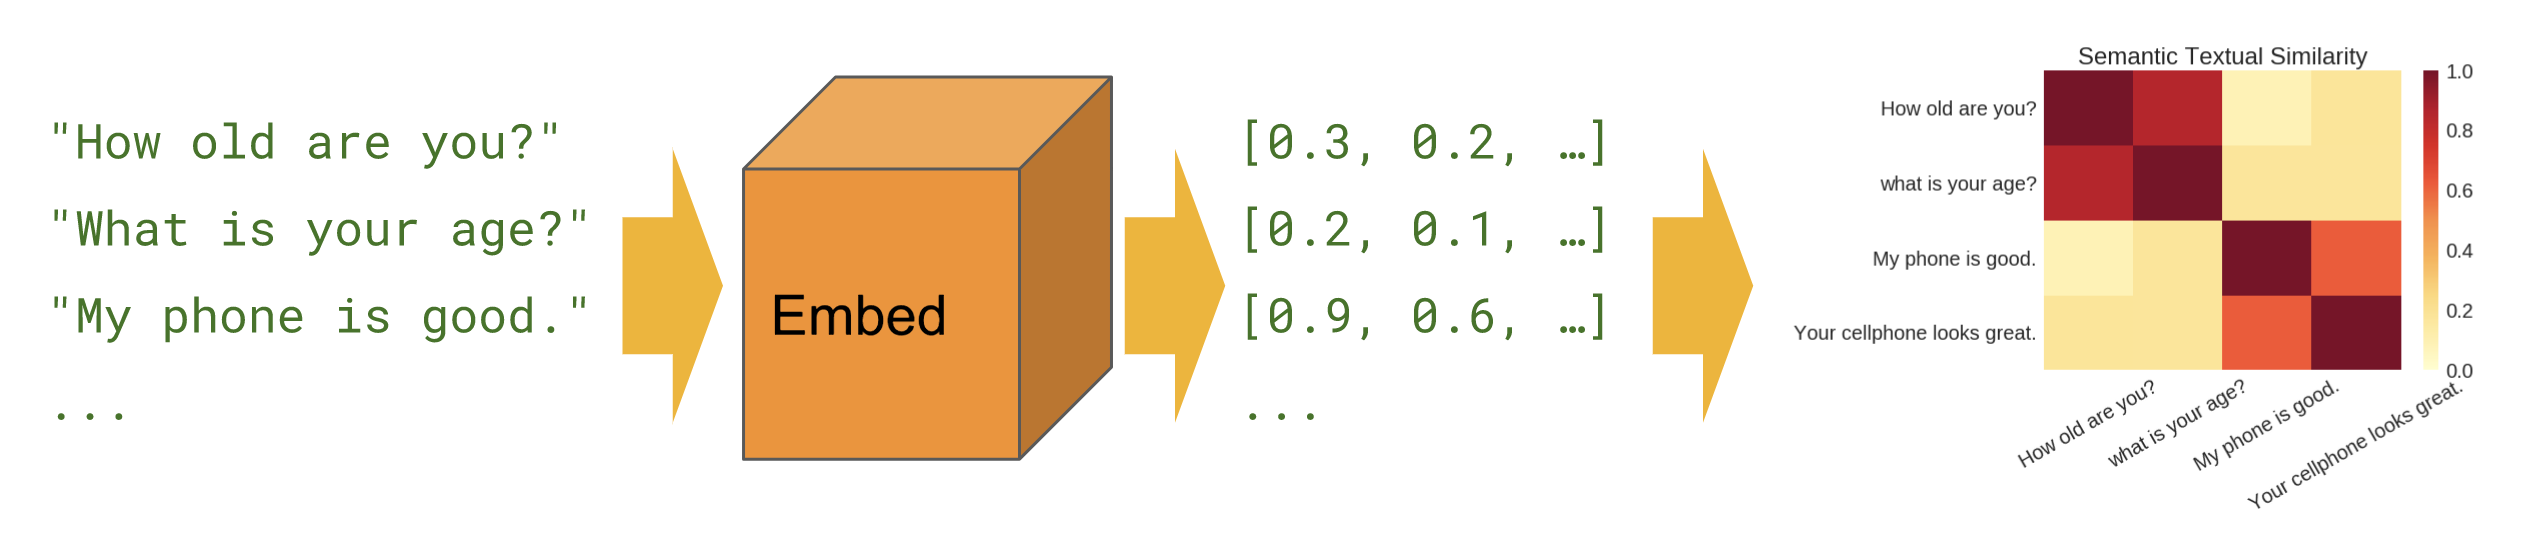
\includegraphics [scale=0.4]{Figure/use.png}
    \caption{Esempio funzionamento USE}
    \label{fig:my_label}
\end{figure}
\FloatBarrier
USE ha vari tipo di encoder, quello utilizzato in questo lavoro è un encoder multilingua che supporta 16 lingue diverse(arabo, cinese-semplificato, cinese-tradizionale, francese, inglese, italiano, giapponese, coreano, olandese, polacco, portoghese, spagnolo, tailandese, turco, russo, tedesco). In questo modo il nostro i modelli che verranno addestrati saranno in grado di riconoscere dati sensibili scritti nelle 16 lingue indicate in precedenza.